\chapter{Postup vytvorenia komponentov}

Spôsob vytvorenia grafických komponentov je nasledovný. Najprv používateľ vytvorí SVG súbor, následne ho načíta a vytvorí funkcie v JavaScripte na ovládanie atribútov SVG elementu. 
Alternatívna možnosť je vytvoriť SVG elementy prostredníctvom JavaScriptovej knižnice a nenačítavať súbor. 

\section{Použitie SVG v HTML dokumente}

SVG sa dá použiť a vytvoriť viacerými spôsobmi:
\begin{itemize}
	\item priamo v HTML dokumente - inline, 
	\item načítanie z oddeleného SVG súboru,
	\item načítanie pomocou JavaScriptovej knižnice.
\end{itemize}

\subsubsection{Postup pri načítaní JavaScript knižnice a SVG súboru}

Postup (načítanie súboru v tele JavaScriptovej metóde): 
\begin{enumerate}
	\item Načítať knižnicu Snap.svg.js do HTML súboru. 
	\item Pridať atribút onPageLoad(); do definicie body.
	\item Pridať HTML tag $<$svg$>$ do tela HTML a nastaviť v ňom požadovanú veľkosť cez viewBox.
	\item Vytvoriť JavaScriptový súbor, alebo tag $<$script$>$, ktorý bude obsahovať funkcie. 
	\item Vytvorenie funkcie na načítanie Snap API a .SVG súboru. 
	\item V tele funkcie inicializácia Snap Canvasu. To znamená, kde konkrétne v HTML stránke sa zobrazí.
	\begin{itemize}
		\item s = Snap() - najbližšie voľné miesto
		\item s = Snap(šírka, výška) 
		\item s = Snap(HTMLtag) - id tagu $<$svg$>$, ktoré sa pridalo v bode č. 3
	\end{itemize}
	\item Načítanie .SVG súboru cez funkciu Snap.load(), s parametrami: názov súboru a funkcie s parametrom f. 
	\item Zobrazenie súboru cez príkaz s.append(f);, ekvivalentné zápisy: s.appendAll(f);, s.add(f);. 
	\item V HTML stránke sa zobrazí daný .SVG súbor. 
	
	
\end{enumerate}

V nasledujúcej časti je postup krokov pre ovládania SVG elementu:

\begin{enumerate}
	\item Vytvorenie novej funkcie. 
	\begin{itemize}
		\item anonymná funkcia 
		\item pomenovaná funkcia
		\item objekt, v ktorom bude zadefinovaná funkcia. 
	\end{itemize}
	\item Nová premenná var, ktorá obsahuje id SVG elementu, ktorý sa ide ovládať. (Na zistenie id SVG viď Postup krokov na zistenie id.)
	\item Vytvorenie funkcie, cez ktorú sa bude pristupovať k API Snap knižnice. 
	\item s.select(id SVG)
	\item V tejto chvíli je možné volať funkcie z Snap.svg API príkazom: element.funkciaAPISnap.. 
	\begin{itemize}
		\item element.animate() - animácia
		\item element.attr() - nastavenie atribútu
		\item element.add(), a iné.	
	\end{itemize}	
\end{enumerate}


V nasledujúcej časti sú zobrazené UML diagramy, ktoré zobrazujú postup načítania, vytvorenia, ovládania grafických komponentov. 

Webový prehliadač dostáva informácie zo SCADA systému, ktoré musí spracovať. Následné zmeny sa dajú animovať a vizualizovať. Na obrázku \ref{fig:USECASE} sú zobrazené možnosti na vizualizáciu. 
	
    V predošlej časti bolo popísané v krokoch ako postupovať pri načítaní SVG súboru. Pre lepšie pochopenie je vytvorený UML diagram aktivít, ktorý popisuje postup načítania SVG. Je zobrazený na obrázku \ref{fig:aktivity1}. 
    
    Pre ovládanie elementu je potrebné zistiť id elementu. Existuje viacero spôsobov, ako to realizovať. Na obrázku \ref{fig:ovladanie} je diagram aktivít. Diagram zobrazuje aj postup ako animovať a meniť atribúty daného elementu. 
    
\begin{figure}[H]
		\centering
		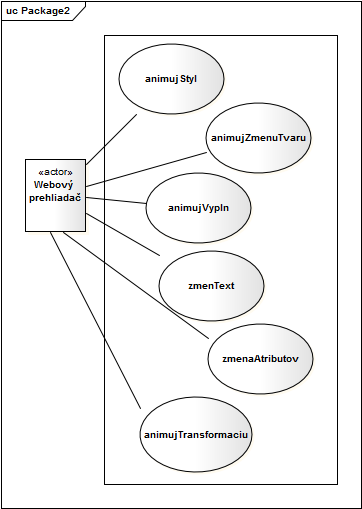
\includegraphics[width=0.4\linewidth]{uml/usecase_update.png}
		\caption{Diagram prípadov použitia vizualizácie v SCADA systémoch}
		\label{fig:USECASE}
	\end{figure}

	
	\begin{figure}[H]
		\centering
		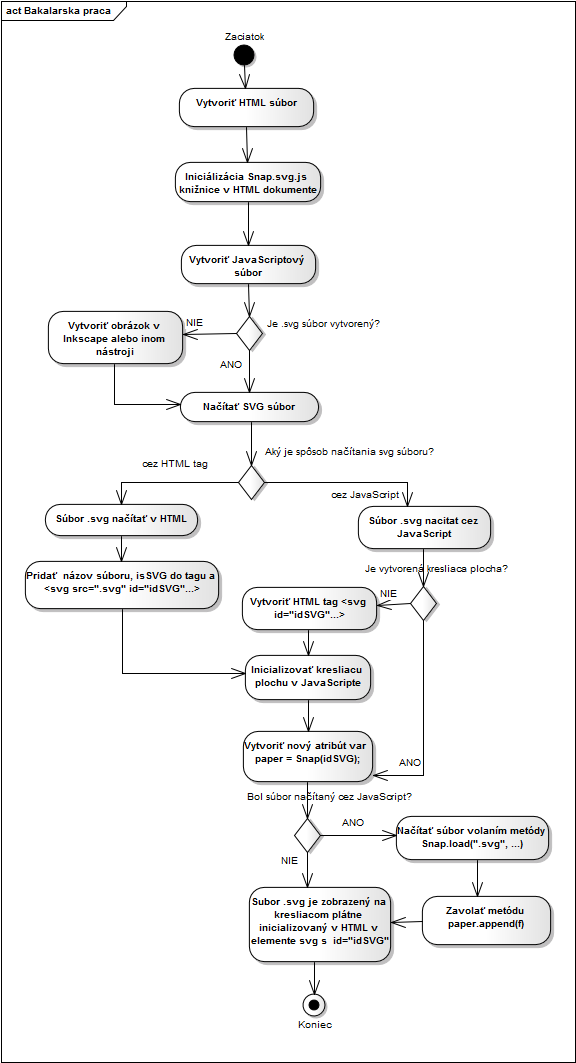
\includegraphics[width=0.6\linewidth]{uml/aktivityInicializacie.png}
		\caption{Postup načítania SVG súboru v HTML dokumente}
		\label{fig:aktivity1}
\end{figure}

\begin{figure}[H]
	\centering
	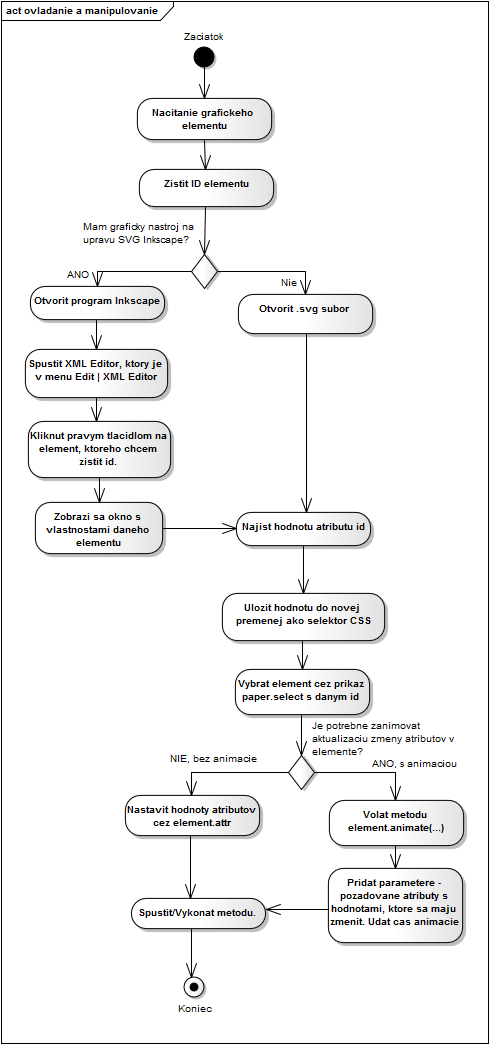
\includegraphics[width=0.6\linewidth]{uml/aktivity2.png}
	\caption{Postup zistenia id elementu a jeho aktualizovanie}
	\label{fig:ovladanie}
\end{figure}